\section{解的流映射}
\label{sec:odesens-flow}

到现在为止我们盯着一条解和它附近的解。换一个视角：固定起止时刻，让所有初始状态同时运动。方向场上每一点都顺流而下，整个状态空间被搬动了一段。这个“搬动”本身是一个映射，前面得到的初值依赖、Jacobian矩阵都成为它的性质。

本节设$\bm{D}\subseteq\mathbb{R}\times\mathbb{R}^{n}$开，$\bm{f}:\bm{D}\to\mathbb{R}^{n}$连续，且$\partial_{\bm{x}}\bm{f}$在$\bm{D}$上存在并连续，这样过$\bm{D}$中每点的最大解都存在且唯一。时间可测时，把$\bm{f}$的条件换成定理~\ref{thm:odesens-differentiable}的条件，并把涉及时间导数的结论理解为几乎处处成立。

\begin{definition}[流映射]
\label{def:odesens-flow}
对时刻$s,t$，记$\bm{D}_{s,t}$为满足下述条件的$\bm{x}\in\mathbb{R}^{n}$的集合：$(s,\bm{x})\in\bm{D}$，且过$(s,\bm{x})$的最大解在时刻$t$有定义。在$\bm{D}_{s,t}$上定义\term{流映射}（flow map）
\begin{equation}
 \bm{\varphi}_{s,t}(\bm{x})=\text{过}(s,\bm{x})\text{的最大解在时刻}\ t\ \text{的值}.
 \label{eq:odesens-flow}
\end{equation}
\end{definition}

记号$\bm{\varphi}_{s,t}$保留了起止两个时刻。$\bm{D}_{s,t}$可能是真子集，甚至是空集，因为有些解活不到$t$。由定理~\ref{thm:odesens-local-lipschitz}，$\bm{D}_{s,t}$是开集，$\bm{\varphi}_{s,t}$在其上局部Lipschitz；由定理~\ref{thm:odesens-differentiable}，它连续可微，Jacobian矩阵是沿相应解的状态转移矩阵，
\begin{equation}
 \mathrm{D}\bm{\varphi}_{s,t}(\bm{x})=\bm{\Phi}(t,s).
 \label{eq:odesens-flow-jacobian}
\end{equation}
图~\ref{fig:odesens-flow-domain}是$\dot{x}=x^2$的流映射，它的定义域随$t$收缩。

\begin{BookInlineFigure}
  \centering
  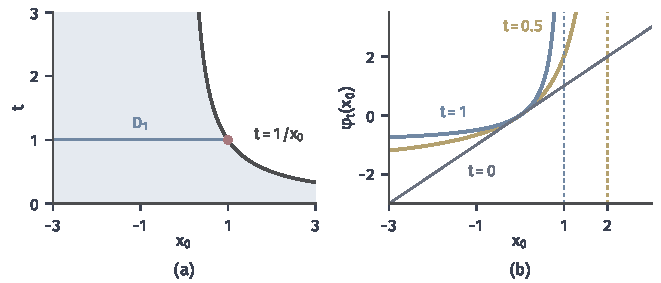
\includegraphics[width=112mm]{figures/06-differential-equations/01-ordinary-differential-equations/matplotlib/odesens-flow-domain/figure.pdf}
  \caption{流映射的定义域依赖时间。方程$\dot{x}=x^2$，$\varphi_t(x)=x/(1-tx)$。(a)浅蓝区域是$\{(x_0,t):t\geq0,\ tx_0<1\}$，深灰线是爆炸曲线$t=1/x_0$，蓝色水平线是$t=1$时的定义域$\bm{D}_1=(-\infty,1)$。(b)$\varphi_t$的图像，$t=0$是恒等映射（灰），$t=0.5$（黄）、$t=1$（蓝）在虚线处趋于无穷。}
  \label{fig:odesens-flow-domain}
\end{BookInlineFigure}

\subsection{局部可逆性}
\label{sec:odesens-flow-inverse}

解在唯一性条件下不会分叉也不会合并。所以从$s$走到$r$再走到$t$，应当等于直接走到$t$；从$s$走到$t$再走回来，应当回到原处。这是流映射的两条代数规则，图~\ref{fig:odesens-flow-composition}是它们的示意。

\begin{BookInlineFigure}
  \centering
  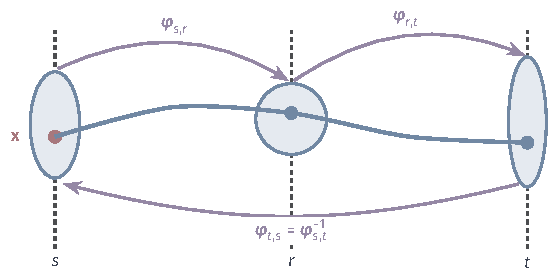
\includegraphics[width=93.4mm]{figures/06-differential-equations/01-ordinary-differential-equations/tikz/odesens-flow-composition/figure.pdf}
  \caption{流映射的复合与逆。三条虚线是时刻$s,r,t$上的状态空间，浅蓝区域是一小块初值及其像，蓝线是过红点的解。上方两个映射相继作用等于$\bm{\varphi}_{s,t}$，下方的映射$\bm{\varphi}_{t,s}$把终点送回起点。}
  \label{fig:odesens-flow-composition}
\end{BookInlineFigure}

\begin{theorem}[流映射的复合与局部可逆性]
\label{thm:odesens-flow}
在本节的条件下：
\begin{enumerate}
 \item 对$(s,\bm{x})\in\bm{D}$，有$\bm{\varphi}_{s,s}(\bm{x})=\bm{x}$；
 \item 若$\bm{x}\in\bm{D}_{s,r}$且$\bm{\varphi}_{s,r}(\bm{x})\in\bm{D}_{r,t}$，则$\bm{x}\in\bm{D}_{s,t}$，且
 \begin{equation}
  \bm{\varphi}_{r,t}\bigl(\bm{\varphi}_{s,r}(\bm{x})\bigr)=\bm{\varphi}_{s,t}(\bm{x});
  \label{eq:odesens-flow-composition}
 \end{equation}
 \item $\bm{\varphi}_{s,t}:\bm{D}_{s,t}\to\bm{D}_{t,s}$是$C^1$双射，逆映射是$\bm{\varphi}_{t,s}$，且Jacobian矩阵处处可逆，
 \begin{equation}
  \mathrm{D}\bm{\varphi}_{t,s}\bigl(\bm{\varphi}_{s,t}(\bm{x})\bigr)=\bigl[\mathrm{D}\bm{\varphi}_{s,t}(\bm{x})\bigr]^{-1}.
  \label{eq:odesens-flow-inverse}
 \end{equation}
\end{enumerate}
\end{theorem}

\begin{proof}
第一条是定义。

第二条用唯一性。过$(s,\bm{x})$的最大解在时刻$r$的值是$\bm{\varphi}_{s,r}(\bm{x})$，所以它也是过$(r,\bm{\varphi}_{s,r}(\bm{x}))$的解。由最大解的唯一性，这两条最大解相同。后者在$t$有定义，前者也就在$t$有定义，两边的值相等。

第三条是第二条的特例。设$\bm{x}\in\bm{D}_{s,t}$，$\bm{y}=\bm{\varphi}_{s,t}(\bm{x})$。过$(t,\bm{y})$的最大解就是过$(s,\bm{x})$的最大解，它在$s$有定义且值为$\bm{x}$，所以$\bm{y}\in\bm{D}_{t,s}$，且$\bm{\varphi}_{t,s}(\bm{y})=\bm{x}$。交换$s,t$得到另一个方向。两个映射都是$C^1$的，对恒等映射$\bm{\varphi}_{t,s}\circ\bm{\varphi}_{s,t}$用链式法则，就得到式~\eqref{eq:odesens-flow-inverse}。
\end{proof}

这里没有用到反函数定理，逆映射是由“反向求解”直接造出来的，并且在整个$\bm{D}_{s,t}$上有定义，不只在一点附近。之所以仍称为局部可逆性，是因为$\bm{D}_{s,t}$通常不是整个空间，定理并不假定解全局存在。

\paragraph{自治方程与单参数局部流}
当$\bm{f}$不显含时间时，若$\bm{x}(t)$是解，平移后的$\bm{x}(t+c)$也是解。于是$\bm{\varphi}_{s,t}$只依赖时长$t-s$，记$\bm{\varphi}_{t}=\bm{\varphi}_{0,t}$。式~\eqref{eq:odesens-flow-composition}变成
\begin{equation}
 \bm{\varphi}_{t}\circ\bm{\varphi}_{r}=\bm{\varphi}_{t+r}.
 \label{eq:odesens-local-flow}
\end{equation}
等式在式~\eqref{eq:odesens-flow-composition}的定义域条件下成立，所以$\{\bm{\varphi}_t\}$称为\term{单参数局部流}（local one-parameter flow）。若所有解全局存在，它才是定义在整个空间上的单参数群。

对$\dot{x}=x^2$，$\varphi_t(x)=x/(1-tx)$，直接代入，
\[
 \varphi_t\bigl(\varphi_r(x)\bigr)=\frac{x/(1-rx)}{1-tx/(1-rx)}=\frac{x}{1-(t+r)x}=\varphi_{t+r}(x),
\]
要求$rx<1$且$tx/(1-rx)<1$。当$t,r>0$时，这等价于$(t+r)x<1$；$\varphi_{-t}$是$\varphi_t$在定义域上的逆。

非自治方程不能这样简写。对$\dot{x}=tx$，$\varphi_{s,t}(x)=x\,\mathrm{e}^{(t^2-s^2)/2}$。从$0$走到$1$乘以$\mathrm{e}^{1/2}$，再用同一规律“走一个单位时间”乘以$\mathrm{e}^{1/2}$，得到的$\mathrm{e}$并不等于从$0$到$2$的倍数$\mathrm{e}^{2}$。第二段时间的起点是$1$，规律已经变了，所以必须记下起止两个时刻。

\paragraph{没有唯一性时会怎样}
可逆性来自轨道不合并。方程$\dot{x}=-2\,\mathrm{sgn}(x)\sqrt{\lvert x\rvert}$在$x=0$处不Lipschitz。正向解唯一：右端单调递减，式~\eqref{eq:odesens-one-sided}成立且$\mu=0$，由引理~\ref{lem:odesens-one-sided}，两条解的距离不增，所以正向唯一。解是
\[
 x(t)=\mathrm{sgn}(x_0)\bigl(\max\{\sqrt{\lvert x_0\rvert}-t,\,0\}\bigr)^2.
\]

所有$\lvert x_0\rvert\leq t^2$的轨道在时刻$t$都已并入$0$，见图~\ref{fig:odesens-merging}。$\varphi_1$把整个$[-1,1]$压成一点，不是单射，没有逆映射，这正是反向解不唯一的表现。

\begin{BookInlineFigure}
  \centering
  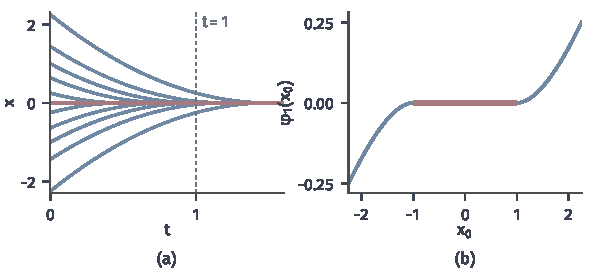
\includegraphics[width=100mm]{figures/06-differential-equations/01-ordinary-differential-equations/matplotlib/odesens-merging/figure.pdf}
  \caption{轨道合并破坏可逆性。方程$\dot{x}=-2\,\mathrm{sgn}(x)\sqrt{\lvert x\rvert}$。(a)各初值的轨道在有限时间并入红色的零解。(b)$t=1$时的解映射，红色线段$[-1,1]$被压成一点。}
  \label{fig:odesens-merging}
\end{BookInlineFigure}

\subsection{体积变化}
\label{sec:odesens-volume}

流映射把一小块初始区域搬到别处，体积会变吗？线性映射的体积倍数是行列式的绝对值，而流映射在一小块上近似线性，Jacobian矩阵是$\bm{S}(t)$。于是要看的是$J(t)=\det\bm{S}(t)$怎样随时间变化。

\paragraph{直观}
考虑很短的时间$h$，由式~\eqref{eq:odesens-initial-variational}有$\bm{S}(t+h)\approx(\bm{I}+h\bm{A}(t))\bm{S}(t)$。而
\[
 \det(\bm{I}+h\bm{A})=1+h\operatorname{tr}\bm{A}+O(h^2),
\]
所以每一小段时间内体积的相对变化率是$\operatorname{tr}\bm{A}$，也就是右端的散度。放在水流的图景中，散度是某点处水流的“膨胀率”：散度为正的地方，流体微团在膨胀。把这个观察写成精确的等式，就是\term{Liouville公式}（Liouville formula）。

\begin{lemma}[Liouville公式]
\label{lem:odesens-liouville}
设$\bm{S}$满足式~\eqref{eq:odesens-initial-variational}，其中$\bm{A}$可积。则$J=\det\bm{S}$绝对连续，几乎处处满足$\dot{J}=\operatorname{tr}\bm{A}(t)\,J$，于是
\begin{equation}
 J(t)=\exp\int_{t_0}^{t}\operatorname{tr}\bm{A}(s)\,\mathrm{d}s>0.
 \label{eq:odesens-liouville}
\end{equation}
\end{lemma}

\begin{proof}
行列式是矩阵元素的多项式，$\bm{S}$绝对连续，所以$J$绝对连续。矩阵函数的微分给出
\[
 \mathrm{d}\det{}_{\bm{S}}(\bm{E})=\operatorname{tr}\bigl(\operatorname{adj}(\bm{S})\bm{E}\bigr),
\]
这个公式对奇异矩阵也成立，可参考\BookChapterRef{chap:matrix-differentiation}{卷二第21章“矩阵函数的微分”}。代入$\dot{\bm{S}}=\bm{A}\bm{S}$，
\[
 \dot{J}=\operatorname{tr}\bigl(\operatorname{adj}(\bm{S})\bm{A}\bm{S}\bigr).
\]

用迹的循环性，再用$\bm{S}$与其古典伴随的乘积等于$\det(\bm{S})\bm{I}$，
\[
 \dot{J}=\operatorname{tr}\bigl(\bm{A}\bm{S}\operatorname{adj}(\bm{S})\bigr)=\operatorname{tr}(\bm{A})\,J.
\]
这是标量线性方程，$J(t_0)=1$，解就是式~\eqref{eq:odesens-liouville}。
\end{proof}

沿解，$\operatorname{tr}\bm{A}(t)$正是右端在$(t,\bm{x}(t))$处的散度$\nabla\cdot\bm{f}$，这里的散度只对状态变量求。式~\eqref{eq:odesens-liouville}中$J>0$说明流映射保持定向，也就不会出现把区域翻折的情况。

三个手算例子可以用来核对。常系数线性方程$\dot{\bm{x}}=\bm{A}\bm{x}$有
\[
 \det\mathrm{e}^{t\bm{A}}=\mathrm{e}^{t\operatorname{tr}\bm{A}}.
\]
例~\ref{ex:odesens-planar}的散度是$-1+1=0$，相应的行列式是$\tfrac12\cdot2=1$。Logistic方程是一维的，“体积”就是长度，放大倍数$\exp\int(1-2x)\,\mathrm{d}t$等于$4/3$，与$S(\ln3)$相同。

\begin{theorem}[体积变化公式]
\label{thm:odesens-volume}
在本节的条件下，设$\bm{W}\subseteq\bm{D}_{s,t}$是可测集。则
\begin{equation}
 \operatorname{vol}\bigl(\bm{\varphi}_{s,t}(\bm{W})\bigr)=\int_{\bm{W}}\exp\Bigl(\int_{s}^{t}\nabla\cdot\bm{f}\bigl(r,\bm{\varphi}_{s,r}(\bm{x})\bigr)\,\mathrm{d}r\Bigr)\mathrm{d}\bm{x}.
 \label{eq:odesens-volume}
\end{equation}
特别地，若$\bm{f}$的定义域$\bm{D}$上$\nabla\cdot\bm{f}\equiv0$，则流映射保持体积。反过来，若流映射对任意$s,t$和任意小球都保持体积，则$\nabla\cdot\bm{f}\equiv0$。
\end{theorem}

\begin{proof}
由定理~\ref{thm:odesens-flow}，$\bm{\varphi}_{s,t}$是开集之间的$C^1$双射，且Jacobian矩阵可逆。换元公式给出
\[
 \operatorname{vol}\bigl(\bm{\varphi}_{s,t}(\bm{W})\bigr)=\int_{\bm{W}}\bigl\lvert\det\mathrm{D}\bm{\varphi}_{s,t}(\bm{x})\bigr\rvert\,\mathrm{d}\bm{x}.
\]
这个公式及测度论背景可参考\BookChapterRef{chap:pushforward-measures}{卷四第9章“推前测度”}。把式~\eqref{eq:odesens-flow-jacobian}、式~\eqref{eq:odesens-liouville}代入，即得式~\eqref{eq:odesens-volume}，绝对值因$J>0$可去。

散度恒为零时，被积函数恒为$1$，体积保持。反过来，设某点$(s,\bm{x})$处$\nabla\cdot\bm{f}>0$（负的情形相同）。由连续性，$(s,\bm{x})$附近散度为正，取小球$\bm{W}$和很短的时间，使轨道段留在这个邻域内，则式~\eqref{eq:odesens-volume}的指数中积分为正，体积严格增大，矛盾。
\end{proof}

定理的条件都起作用。解的唯一性保证$\bm{\varphi}_{s,t}$单射，否则换元公式就不再有意义，图~\ref{fig:odesens-merging}的压缩映射便是反例。$\bm{f}$关于状态$C^1$保证了$\mathrm{D}\bm{\varphi}$连续。结论仅对$\bm{W}\subseteq\bm{D}_{s,t}$成立，爆炸的解所在的点不在其中。

图~\ref{fig:odesens-volume-change}比较了三种流。例~\ref{ex:odesens-planar}的流把正方形拉成细长曲边四边形，面积不变。阻尼振子$\dot{q}=p$、$\dot{p}=-q-\tfrac12p$的散度是$-\tfrac12$，面积按$\mathrm{e}^{-t/2}$缩小，边长$0.5$的正方形面积$0.25$，$t=2$时为$0.25\,\mathrm{e}^{-1}\approx0.092$。

\begin{BookInlineFigure}
  \centering
  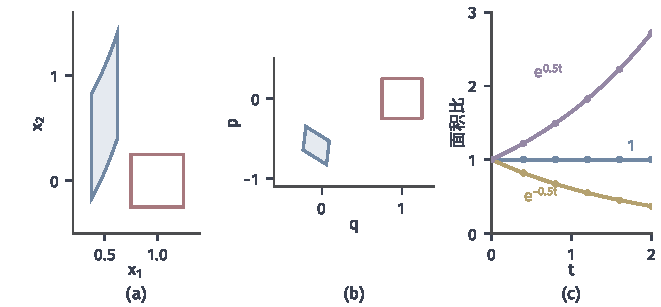
\includegraphics[width=112mm]{figures/06-differential-equations/01-ordinary-differential-equations/matplotlib/odesens-volume-change/figure.pdf}
  \caption{面积随流的变化。红框是初始正方形，浅蓝区域是它的像。(a)$\dot{x}_1=-x_1$、$\dot{x}_2=x_2+x_1^2$，$t=\ln2$，散度为零。(b)$\dot{q}=p$、$\dot{p}=-q-\tfrac12p$，$t=2$，散度为$-\tfrac12$。(c)面积比随时间的变化：线是式~\eqref{eq:odesens-liouville}，点是由多边形面积算出的数值；蓝、黄分别对应(a)(b)，紫色对应$\dot{\bm{x}}=\tfrac14\bm{x}$。}
  \label{fig:odesens-volume-change}
\end{BookInlineFigure}

\paragraph{沿轨迹的值与密度}
一块墨水随水流运动，某个粒子携带的值沿轨迹不变，而墨水的密度要随微团的伸缩改变，这是两件不同的事。设质量密度$p_s$在流映射下被推到$p_t$，质量守恒要求对任意$\bm{W}$有
\[
 \int_{\bm{\varphi}_{s,t}(\bm{W})}p_t(\bm{y})\,\mathrm{d}\bm{y}=\int_{\bm{W}}p_s(\bm{x})\,\mathrm{d}\bm{x}.
\]
左边用换元公式换回$\bm{x}$，比较被积函数，得到
\begin{equation}
 p_t\bigl(\bm{\varphi}_{s,t}(\bm{x})\bigr)=\frac{p_s(\bm{x})}{\det\mathrm{D}\bm{\varphi}_{s,t}(\bm{x})}.
 \label{eq:odesens-density}
\end{equation}
取对数并对$t$求导，由式~\eqref{eq:odesens-liouville}，沿轨迹有
\[
 \frac{\mathrm{d}}{\mathrm{d}t}\ln p_t\bigl(\bm{x}(t)\bigr)=-\nabla\cdot\bm{f}\bigl(t,\bm{x}(t)\bigr).
\]
膨胀的地方密度下降。

以Logistic方程为例。$x_0$在$[0.1,0.4]$上均匀分布，密度$p_0=10/3$。$T=\ln3$时，$x_0=1/4$被送到$1/2$，Jacobian是$4/3$，所以
\[
 p_T(1/2)=\frac{10/3}{4/3}=2.5.
\]
图~\ref{fig:odesens-density-push}对比了这个公式与样本直方图。右侧的$x_0$被拉伸得少，密度更高。式~\eqref{eq:odesens-density}是第~\ref{chap:transport-equations}章输运方程的基础，随机变量经可逆映射变换时的密度公式也是同一件事，可参考\BookChapterRef{chap:random-sampling-integration}{卷七第14章“随机采样与积分计算”}。

\begin{BookInlineFigure}
  \centering
  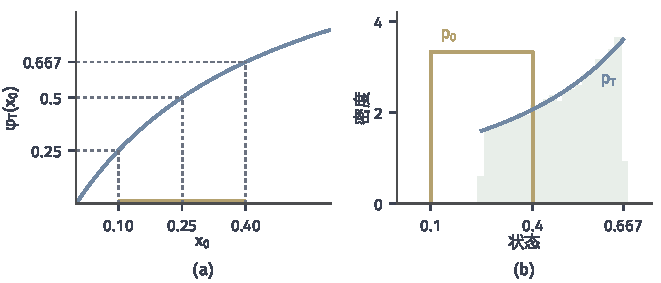
\includegraphics[width=112mm]{figures/06-differential-equations/01-ordinary-differential-equations/matplotlib/odesens-density-push/figure.pdf}
  \caption{流映射推动密度。方程$\dot{x}=x(1-x)$，$T=\ln3$。(a)流映射把黄色区间$[0.1,0.4]$送到$[0.25,0.667]$。(b)均匀密度$p_0$（黄）被推成$p_T$（蓝），绿色直方图来自$40000$个由固定种子生成的样本。}
  \label{fig:odesens-density-push}
\end{BookInlineFigure}

\subsection{Hamilton流}
\label{sec:odesens-hamilton}

有一类重要的方程，散度为零是结构带来的，不用逐个验证。力学系统的状态由位置$\bm{q}$和动量$\bm{p}$组成，运动由一个函数决定。摆的总能量是$H(q,p)=\tfrac12p^2+1-\cos q$，而摆的方程$\dot{q}=p$、$\dot{p}=-\sin q$恰好是
\[
 \dot{q}=\partial_pH,\qquad \dot{p}=-\partial_qH.
\]
这个形式可以推广。

\begin{definition}[Hamilton方程]
\label{def:odesens-hamilton}
设$H(t,\bm{q},\bm{p})$是定义在$\mathbb{R}\times\mathbb{R}^{m}\times\mathbb{R}^{m}$的开集上的函数，关于$t$连续，关于$(\bm{q},\bm{p})$二阶连续可微，且这些偏导数连续。称
\begin{equation}
 \dot{\bm{q}}=\nabla_{\bm{p}}H(t,\bm{q},\bm{p}),\qquad
 \dot{\bm{p}}=-\nabla_{\bm{q}}H(t,\bm{q},\bm{p})
 \label{eq:odesens-hamilton}
\end{equation}
为\term{Hamilton方程}（Hamilton's equations），$H$称为Hamilton函数（Hamiltonian），$(\bm{q},\bm{p})\in\mathbb{R}^{2m}$所在空间称为\term{相空间}（phase space），相应的流映射称为\term{Hamilton流}（Hamiltonian flow）。
\end{definition}

$H\in C^2$正好保证右端关于状态$C^1$，本节前面的结论全部适用。下面两条性质分别回答体积和能量。

\begin{theorem}[Hamilton流的体积与能量]
\label{thm:odesens-hamilton}
在定义~\ref{def:odesens-hamilton}的条件下，Hamilton流在其定义域内保持相空间体积（$H$可以显含时间）。若$H$还关于$t$连续可微，沿Hamilton方程的解有
\begin{equation}
 \frac{\mathrm{d}}{\mathrm{d}t}H\bigl(t,\bm{q}(t),\bm{p}(t)\bigr)=\partial_tH\bigl(t,\bm{q}(t),\bm{p}(t)\bigr).
 \label{eq:odesens-energy}
\end{equation}
特别地，$H$不显含时间时，$H$沿解不变。
\end{theorem}

\begin{proof}
相空间中的散度是
\[
 \nabla\cdot\bm{f}=\sum_{i=1}^{m}\Bigl(\frac{\partial}{\partial q_i}\frac{\partial H}{\partial p_i}-\frac{\partial}{\partial p_i}\frac{\partial H}{\partial q_i}\Bigr)=0,
\]
最后一步用了$H\in C^2$时混合偏导相等。由定理~\ref{thm:odesens-volume}，流保持体积。

由链式法则及式~\eqref{eq:odesens-hamilton}，
\[
 \frac{\mathrm{d}H}{\mathrm{d}t}=\partial_tH+\langle\nabla_{\bm{q}}H,\dot{\bm{q}}\rangle+\langle\nabla_{\bm{p}}H,\dot{\bm{p}}\rangle=\partial_tH+\langle\nabla_{\bm{q}}H,\nabla_{\bm{p}}H\rangle-\langle\nabla_{\bm{p}}H,\nabla_{\bm{q}}H\rangle.
\]
后两项相消，即得式~\eqref{eq:odesens-energy}。
\end{proof}

显含时间时，能量可以变化。受迫振子取$H=\tfrac12p^2+\tfrac12q^2-g(t)q$，方程是$\dot{q}=p$、$\dot{p}=-q+g(t)$，式~\eqref{eq:odesens-energy}的右端是$-\dot{g}(t)q$。取$g(t)=t$，$q(0)=0$，$p(0)=1$，解是$q=t$、$p=1$，代入$H$得
\[
 H(t,t,1)=\tfrac12+\tfrac12t^2-t^2=\tfrac12-\tfrac12t^2.
\]
其导数是$-t$，正好等于$-\dot{g}q=-t$。此时能量不守恒，但相空间体积仍然保持。

图~\ref{fig:odesens-hamilton-flow}是摆的相空间。在无阻尼情形下，半径$0.35$的圆被剪切成细长的月牙形，沿能量等值线运动，面积在$t=0,3,6$时都是$0.3848$。加上阻尼$\dot{p}=-\sin q-0.4p$后，方程不再是Hamilton方程，散度为$-0.4$，面积按$\mathrm{e}^{-0.4t}$缩小到$0.1159$与$0.0349$。

\begin{BookInlineFigure}
  \centering
  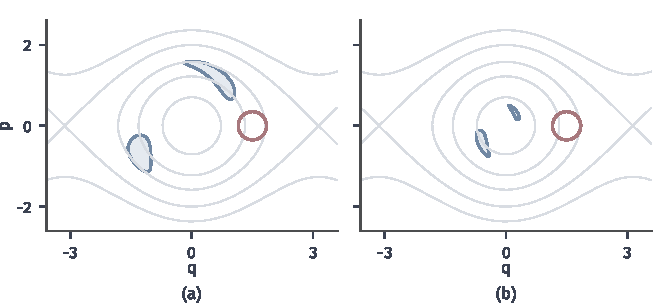
\includegraphics[width=112mm]{figures/06-differential-equations/01-ordinary-differential-equations/matplotlib/odesens-hamilton-flow/figure.pdf}
  \caption{摆的相空间。灰线是能量$H=\tfrac12p^2+1-\cos q$的等值线，红圆是初始区域，浅蓝区域是$t=3$和$t=6$时的像。(a)无阻尼，面积保持。(b)阻尼系数$0.4$，面积按$\mathrm{e}^{-0.4t}$收缩，区域离开能量等值线向内运动。}
  \label{fig:odesens-hamilton-flow}
\end{BookInlineFigure}

体积保持和能量守恒是两个不同的性质，互相不能推出，见表~\ref{tab:odesens-volume-energy}。

\begin{BookInlineTable}
  \centering
  \caption{体积保持与能量守恒的对比。“能量”指表中给定的函数。}
  \label{tab:odesens-volume-energy}
  \begin{tabular}{p{52mm}p{14mm}p{30mm}}
    \toprule
    系统 & 体积 & 能量 \\
    \midrule
    自治Hamilton方程 & 保持 & 守恒 \\
    显含时间的Hamilton方程 & 保持 & 按$\partial_tH$变化 \\
    阻尼摆 & 收缩 & $H$单调不增 \\
    $\dot{q}=(1+q^2)p$，$\dot{p}=-(1+q^2)q$ & 不保持 & $q^2+p^2$守恒 \\
    \bottomrule
  \end{tabular}
\end{BookInlineTable}

表中最后一行的散度是$2qp$，非零，但
\[
 \frac{\mathrm{d}}{\mathrm{d}t}(q^2+p^2)=2(1+q^2)(qp-pq)=0.
\]
这样的方程沿能量面运动，却不保持体积。

Hamilton流的这两条性质是后面几处的基础。第~\ref{chap:hamilton-jacobi-equations}章由Hamilton方程构造特征线，用它们重建场。构造采样提议时，流的可逆性和体积保持让接受概率的计算得以简化，可参考\BookChapterRef{chap:discrete-time-stochastic-processes}{卷九第3章“离散时间随机过程”}。两者都不说明解会靠拢，能量不变也不能推出渐近收敛。
